\documentclass[12pt]{article}
\usepackage[a4paper]{geometry}
\usepackage{fullpage}
\usepackage[T1]{fontenc}
\usepackage[utf8]{inputenc}
\usepackage{graphicx}
\usepackage{mathpazo}
\pagenumbering{gobble}
\usepackage{steinmetz}
\usepackage{siunitx}
\sisetup{output-decimal-marker = {,}}
\usepackage{amsmath}
\usepackage{esdiff}
\usepackage[spanish]{babel}
\newcommand{\laplace}[1]{\mathbf{#1}(\mathbf{s})}
\newcommand{\slp}{\mathbf{s}}

\begin{document}

\title{\textsc{Teoría de Circuitos III}\\Examen Convocatoria Extraordinaria}

\date{25 de junio de  2019}

\maketitle

\subsection*{Instrucciones}
\begin{itemize}
\item El examen tiene una duración de 3 horas.
\item Cada problema se deberá entregar en hojas separadas. No olvides cumplimentar tu número de matrícula, nombre y apellidos en todas las hojas. Las hojas de enunciados \textbf{no} se recogen.
\item La calificación del examen es el promedio de las calificaciones
  de cada problema. Todos los problemas tienen el mismo peso en la
  calificación.
\item Los resultados se publicarán el 28 de junio.La revisión del
  examen se realizará los días \textbf{2 y 4} de julio de
  \textbf{15:30h a 17:30h}.
\end{itemize}

\clearpage

\section*{Ejercicio 1}

El interruptor del circuito de la figura ha permanecido abierto un tiempo elevado, y se cierra en $t = 0$. En estas condiciones debes realizar el siguiente itinerario:

\begin{enumerate}
\item (\textbf{0,5p.}) Determinar las condiciones iniciales de las variables $u_C(0^+)$, $i_L(0^+)$, $i_R(0^+)$.
\item (\textbf{0,5p.}) Determinar los valores en régimen permanente de las variables $u_C(\infty)$, $i_L(\infty)$, $i_R(\infty)$.
\item (\textbf{4p.}) Dibujar el circuito en el dominio de Laplace para $t > 0$, y resolverlo para obtener las expresiones analíticas de $\laplace{I_L}$, $\laplace{U_C}$, $\laplace{I_R}$.
\item (\textbf{1p.}) Comprobar mediante los teoremas de valor inicial y valor final que las expresiones anteriores se ajustan a los resultados de los apartados 1 y 2.

\item (\textbf{1p.}) A partir de las expresiones obtenidas en el apartado 3, indica de forma razonada el tipo de transitorio existente en el circuito.

\item (\textbf{3p.}) Expresión de la variable $i_R(t)$ en el dominio del tiempo.
\end{enumerate}

\begin{minipage}{0.3\textwidth}
Datos:
\begin{align*}
  E_g &= \SI{4}{\volt}\\
  R_1&= \SI{2}{\ohm}\\
  L &= \SI{1}{\henry}\\
  C &= \SI{250}{\milli\farad}\\
  R_2 &= \SI{2}{\ohm}
\end{align*}
\end{minipage}
\begin{minipage}{0.7\textwidth}
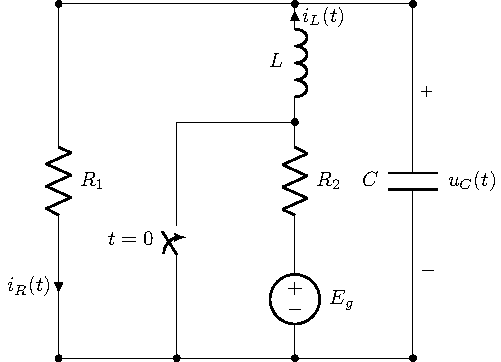
\includegraphics{figs/E2_circuito_v2.pdf}
\end{minipage}

\subsection*{Solución}

\begin{enumerate}
\item

  \begin{align*}
    u_c(0^+) &= \SI{2}{\volt}\\
    i_L(0^+) &= \SI{1}{\ampere}\\
    i_R(0^+) &= \SI{1}{\ampere}
  \end{align*}
  
\item
  \begin{align*}
    u_c(\infty) &= \SI{0}{\volt}\\
    i_L(\infty) &= \SI{0}{\ampere}\\
    i_R(\infty) &= \SI{0}{\ampere}
  \end{align*}
  
\item
  \begin{align*}
    \laplace{I_R} &= \frac{\slp + 2}{\slp^2 + 2\slp + 4}\\
    \laplace{I_L} &= \frac{\slp}{\slp^2 + 2\slp + 4}\\
    \laplace{U_C} &= \frac{2\slp + 4}{\slp^2 + 2\slp + 4}
  \end{align*}
\item
  
  Los resultados del teorema de valor inicial son:

  \begin{align*}
    \lim_{s \to \infty} \slp \laplace{I_L} = i_L(0^+) &= \SI{1}{\ampere}\\
    \lim_{s \to \infty} \slp \laplace{I_R} = i_R(0^+) &= \SI{1}{\ampere}\\
    \lim_{s \to \infty} \slp \laplace{U_C} = u_c(0^+) &= \SI{2}{\volt}\\
  \end{align*}

  Los resultados del teorema de valor final son:

  \begin{align*}
    \lim_{s \to 0} \slp \laplace{I_L} = i_L(\infty) &= \SI{0}{\ampere}\\
    \lim_{s \to 0} \slp \laplace{I_R} = i_R(\infty) &= \SI{0}{\ampere}\\
    \lim_{s \to 0} \slp \laplace{U_C} = u_C(\infty) &= \SI{0}{\volt}\\
  \end{align*}

  Estos resultados corresponden con los obtenidos en los apartados 1 y 2.
\item

  El polinomio del denominador tiene raíces complejas conjugadas ($-1 \pm j \sqrt{3}$), de forma que se trata de un transitorio subamortiguado.
  
\item
  
  \begin{align*}
    i_R(t) &= e^{- t} (\cos(\sqrt{3} t) + \sqrt{3}/3 \sin(\sqrt{3} t))\\
           &= \frac{2\sqrt{3}}{3} e^{- t} \sin(\sqrt{3} t + \ang{60})
  \end{align*}
    
\end{enumerate}

\clearpage

\section*{Ejercicio 2}

En este ejercicio se analizará el comportamiento en frecuencia del circuito de la figura.


\begin{enumerate}

\item (\textbf{4p.}) Determina la función de transferencia en el dominio de Laplace
  \[
    \laplace{H} = \frac{\laplace{V_2}}{\laplace{V_1}}
  \]
  
\item (\textbf{1p.}) A partir de la expresión anterior, obtén la expresión normalizada de la función de transferencia en el dominio de la frecuencia, $\mathbf{H}(\omega)$. 

\item (\textbf{1p.}) Determina la pulsación a la que se encuentran los polos y ceros del sistema.

\item (\textbf{4p.}) Dibuja el diagrama de Bode de \textbf{amplitud y de fase}. ¿Qué tipo de filtro es este circuito?

\end{enumerate}

\begin{minipage}{0.3\textwidth}
Datos:
\begin{align*}
  C &= \SI{170}{\nano\farad}\\
  L &= \SI{30}{\milli\henry}\\
  R_L &= \SI{1}{\ohm}
\end{align*}
\end{minipage}
\begin{minipage}{0.7\textwidth}
  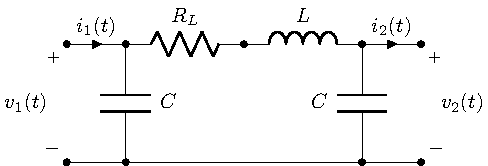
\includegraphics{figs/circuito_respuesta_frecuencia.pdf}
\end{minipage}

\subsection*{Solución}

    \[
      \laplace{H} = \frac{\laplace{V_2}}{\laplace{V_1}} = \frac{1}{\slp^2 LC + \slp RC + 1}
    \]

    \[
      \laplace{H} = \frac{1}{5.1\cdot10^{-9} \slp^2 + 1.7\cdot10^{-7} \slp + 1}
    \]

    Sustituyendo valores numéricos, y reordenando comprobamos que la función se ajusta a la expresión:
      \[
        \mathbf{H}(\omega) = \frac{1}{1 + 2\zeta \frac{\omega}{\omega_o} - (\frac{\omega}{\omega_o})^2}
      \]
      siendo $\zeta = 1.19\cdot10^{-3}$ y $\omega_o= \SI{14002.8}{\radian\per\second}$.
      Esta expresión corresponde a un polo cuadrático en $\omega_o$, y ningún cero. Por tanto, se trata de un filtro paso bajo.

\clearpage

\section*{Ejercicio 3}

En este ejercicio se analizará el comportamiento en resonancia del circuito de la figura. Este circuito está alimentado con una fuente de tensión sinusoidal de valor eficaz $V_g = \SI{100}{\volt}$ y frecuencia $f = \SI{1}{\kilo\hertz}$. El condensador de salida tiene una capacidad de $C = \SI{50}{\nano\farad}$.

\begin{center}
  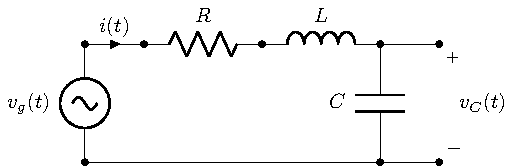
\includegraphics{figs/circuito_resonancia.pdf}
\end{center}

\begin{enumerate}

\item  (\textbf{2,5p.}) Determina la inductancia necesaria para que el circuito entre en resonancia a la frecuencia del generador.

\item  (\textbf{2,5p.}) Determina la resistencia necesaria para obtener una tensión en el condensador de $V_c = \SI{12}{\kilo\volt}$.
  
\item  (\textbf{2,5p.}) A partir de los valores de $L$ y $R$ obtenidos, determina el ancho de banda del circuito y las frecuencias de potencia mitad.

\item  (\textbf{2,5p.}) La frecuencia del generador tiene una tolerancia de $\pm1\%$. Manteniendo los valores de $L$ y $R$ obtenidos en los apartados 1 y 2, determina el valor eficaz de la corriente y la tensión en el condensador en los valores extremos de esta tolerancia.
  
\end{enumerate}

\subsection*{Solución}

\begin{enumerate}
\item 

  \[
    L = \frac{1}{\omega_o^2 C} = \SI{0.506}{\henry}
  \]
  
\item

  \[
    U_c = Q_o U_R = \SI{12}{\kilo\volt}
  \]

  Por tanto, $Q_o = 120$. Al tratarse de un circuito serie RLC:

  \[
    R = \frac{\omega_o L}{Q_o} = \SI{26.53}{\ohm}
  \]
    
\item

  \[
    B = \frac{R}{L} = \SI{52.36}{\radian\per\second}
  \]

  Al ser un circuito con alto factor de calidad, se puede aproximar:

  \begin{align*}
    \omega_1 = \omega_o - B/2 &= \SI{6257}{\radian\per\second}\\
    \omega_2 = \omega_o + B/2 &= \SI{6309}{\radian\per\second}\\
  \end{align*}
\item

  Usamos la curva universal de resonancia con $\epsilon = 0.001$ y $Q_o = 120$. Con $x = Q_o \cdot \epsilon = 1.2$ obtenemos

  \[
    Y(x) = \frac{1}{\sqrt{1 + 4 x^2}} = 0.384
  \]

  La corriente en $\omega_o$ es $I_o = U_g/R = \SI{3.77}{\ampere}$. Por tanto, dentro de esta tolerancia la corriente bajará hasta $\SI{1.46}{\ampere}$, y la tensión en el condensador será $\SI{4.62}{\kilo\volt}$.
\end{enumerate}

\clearpage

\section*{Ejercicio 4}

El cuadripolo $Q$ puede modelarse como la asociación de dos cuadripolos $Q_L$ y $Q_{RC}$. 
\begin{enumerate}

\item (\textbf{1,5p.}) Indica el tipo de asociación, dibuja los circuitos necesarios para comprobar si existe interacción entre los cuadripolos (test de Brune), y razona el resultado que se obtendría.

\item (\textbf{2,5p.}) Determina los parámetros de los cuadripolos $Q_L$ y $Q_{RC}$ más adecuados al tipo de asociación indicado en el apartado anterior. 
\item (\textbf{1p.}) A partir de lo obtenido en el apartado anterior, determina los parámetros del cuadripolo $Q$ como asociación de $Q_L$ y $Q_{RC}$.

\item (\textbf{2,5p.}) Determina los parámetros de transmisión de un cuadripolo equivalente, $Q_T$, conformado por la asociación en cascada de dos cuadripolos $Q$. 

\item (\textbf{2,5p.}) Determina la impedancia que habría que conectar a la salida del cuadripolo $Q_T$ para que desde la entrada de $Q_T$ se observe esa misma impedancia. En estas condiciones, ¿que relación de atenuación hay entre los valores eficaces de las tensiones de entrada y salida del cuadripolo $Q_T$?.
\end{enumerate}


\begin{minipage}{0.2\textwidth}
  Datos:
  \begin{itemize}
  \item $R$ = \SI{2}{\ohm}
  \item $X_C$ = \SI{0.5}{\ohm}
  \item $X_L$ = \SI{2}{\ohm}
  \end{itemize}
\end{minipage}
\begin{minipage}{0.8\textwidth}
  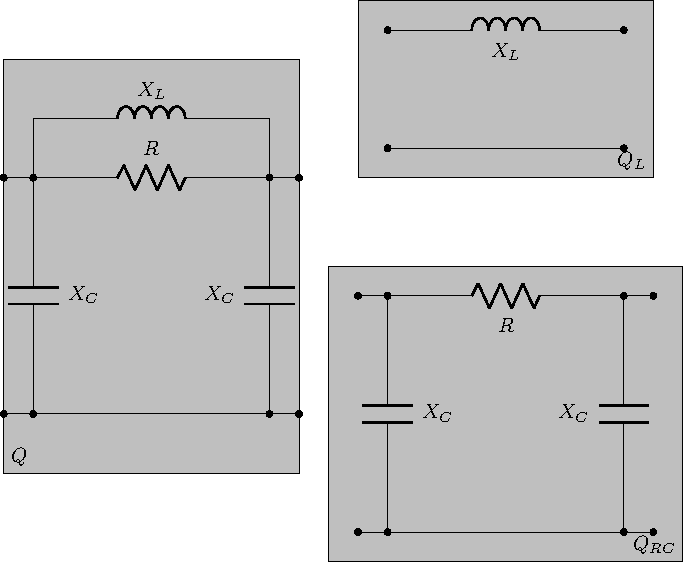
\includegraphics{figs/Cuadripolo_T_puenteada.pdf}
\end{minipage}

\subsection*{Solución}

\begin{enumerate}
\item

  Se trata de una asociación paralelo-paralelo.

  Dado que los dos circuitos tienen un cortocircuito en la línea inferior, no habrá interacción (cumple test de Brune).
\item

  Los parámetros más adecuados son los admitancia.

  \[
  [\overline{Y}_L] = 
  \left[
    \begin{array}{cc}
       -0.5j &  0.5j\\
      0.5j & -0.5j\\
    \end{array}
  \right]
\]

\[
  [\overline{Y}_{RC}] = 
  \left[
    \begin{array}{cc}
      0.5+2j & -0.5\\
      -0.5 & 0.5+2j\\
    \end{array}
  \right]
\]
\item
  \[
  [\overline{Y}_Q] = 
  \left[
    \begin{array}{cc}
      0.5+1.5j & -0.5+0.5j\\
      -0.5+0.5j & 0.5+1.5j\\
    \end{array}
  \right]
\]
\item
\[
  [\overline{T}_Q] = 
  \left[
    \begin{array}{cc}
      -1+2j & 1+j\\
      -4 & -1+2j\\
    \end{array}
  \right]
\]

  \[
    [\overline{T}_{QT}] = [\overline{T}_Q] \cdot [\overline{T}_Q] =
  \left[
    \begin{array}{cc}
      -8-8j & -6+2j\\
      8-16j & -7-8j\\
    \end{array}
  \right]
\]

\item
  Se trata de conectar la impedancia característica del cuadripolo:

  \[
    \overline{Z}_o = \sqrt{\frac{B}{C}} = \SI[parse-numbers=false]{0.595\phase{\ang{-67.5}}}{\ohm}
  \]
  donde se ha escogido el signo positivo de la solución, dado que proporciona una impedancia de resistencia positiva.

  Al conectar esta impedancia, la relación entre las tensiones de entrada y salida está definida por la constante de propagación:

  \[
    \exp{\overline{\gamma}} = \overline{A} + \frac{\overline{B}}{\overline{Z}_o} = -13.97 - 16.04j
  \]

  La relación de atenuación de los valores eficaces de tensión se determina con la parte real de $\overline{\gamma} = \alpha + j\beta$:

  \[
    \exp{\alpha} = \frac{U_1}{U_2} = 21.27
  \]
  
\end{enumerate}


\end{document}

% Local Variables:
% ispell-local-dictionary: "castellano"
% End:

